\documentclass[aspectratio=1610]{beamer}

\usetheme{unnslides}
\usefonttheme{professionalfonts}

\usepackage{listings}
\usepackage{graphicx}
\usepackage{caption}
\usepackage{cmbright}
\usepackage{fontspec}
\usepackage{unicode-math}
\usepackage{amsfonts}
\usepackage{subfig}
\usepackage{tikz}

\captionsetup[subfigure]{labelformat=empty}
\captionsetup[figure]{labelformat=empty}

\setromanfont{CMU Serif}
%\setsansfont{CMU Sans Serif}
\setmathfont{Latin Modern Math}

\usepackage{polyglossia}
%\setbeamertemplate{itemize item}{\color{black}$\blacktriangleright$}

\DeclareMathOperator*{\argmax}{arg\,max}
\DeclareMathOperator*{\argmin}{arg\,min}
\DeclareMathOperator{\sign}{sign}
\DeclareMathOperator{\re}{Re}

\graphicspath{ {../pictures/}{img/} }
%set pages numeration
\setbeamertemplate{footline}[frame number]
\setbeamertemplate{headline}{}
\setlength\abovecaptionskip{-1pt}

\title{Comparison of dimensionality reduction schemes for derivative-free global optimization algorithms}
\author{\textbf{Vladislav~Sovrasov}}
\institute{Lobachevsky State University of Nizhni Novgorod}
\date{}

\begin{document}
\begin{frame}[noframenumbering,plain]
\titlepage
\end{frame}

\begin{frame}
  \frametitle{Problem statement}
  \begin{columns}
    \begin{column}{0.5\textwidth}
      \begin{displaymath}
        \begin{array}{cr}\\
          \varphi(y^*)=\min\{\varphi(y):y\in D\}, \\
          D=\{y\in \mathbb{R}^N:a_i\leq y_i\leq{b_i}, 1\leq{i}\leq{N}\}
        \end{array}
      \end{displaymath}
      \(\varphi(y)\) is multiextremal objective function, which satisfies the Lipschitz condition:
      \begin{displaymath}
        |\varphi(y_1)-\varphi(y_2)|\leq L\Vert y_1-y_2\Vert,y_1,y_2\in D,
      \end{displaymath}
      where \(L>0\) is the Lipschitz constant, and \(||\cdot||\) denotes \(l_2\) norm in \(\mathbb{R}^N\)
      space.
    \end{column}
    \begin{column}{0.5\textwidth}
      \centerline{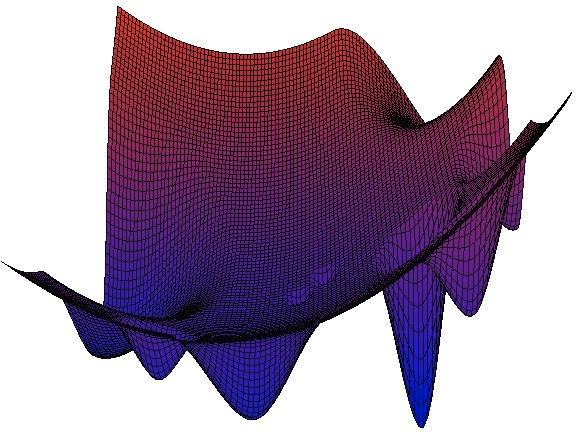
\includegraphics[width=0.9\textwidth]{img/gkls.png}}
    \end{column}
  \end{columns}
\end{frame}

\begin{frame}
  \begin{center}


  \frametitle{Dimension reduction}
  Peano-type curve \(y(x)\) allows to reduce the dimension of the original problem:
  \begin{gather}
    \lbrace y\in \mathbb{R}^N:-2^{-1}\leqslant y_i\leqslant 2^{-1},1\leqslant i\leqslant N\rbrace=\{y(x):0\leqslant x\leqslant 1\} \nonumber \\
    \min\{f(y): y\in D\}=\min\{f(y(x)): x\in [0,1]\} \nonumber
  \end{gather}
  \(y(x)\) is non-smooth function which continuously maps the segment \([0,1]\) to the hypercube \(D\).
  \begin{figure}[ht]
    \vspace*{-0.5cm}
    \subfloat{{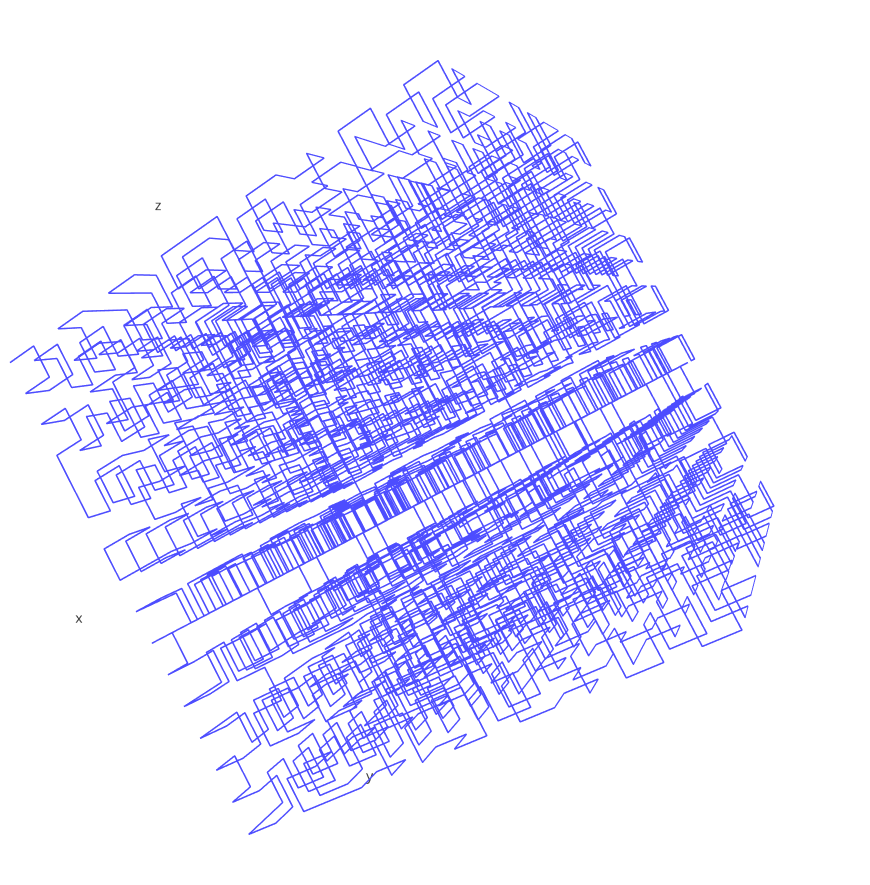
\includegraphics[width=.35\textwidth]{peano3d.png} }}
    \subfloat{{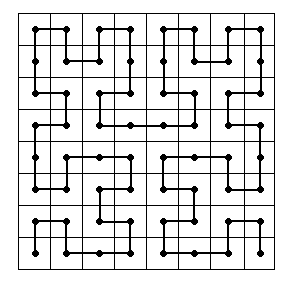
\includegraphics[width=.35\textwidth]{peano2d.png} }}
  \end{figure}
\end{center}
\end{frame}

\begin{frame}
  \frametitle{Properties of the reduced problem}
  After applying the Peano-type evolvent \(\varphi(y(x))\) satisfies the uniform H{\"o}lder condition:
  \begin{displaymath}
    |\varphi(y(x_1))-\varphi(y(x_2))|\leq H{|x_1-x_2|}^{\frac{1}{N}}, x_1,x_2\in[0,1],
  \end{displaymath}
  \(\varphi(y(x))\) is non-smooth and has multiple local extremums even if \(\varphi(y)\) is unimodal.
  The latter problem is caused by loss of the information about \(N\)-d neighborhood after the transformation to the \(1\)-d space.

  \begin{figure}[ht]
    \begin{center}

    \vspace*{-0.5cm}
    \subfloat{\raisebox{.02\textheight}{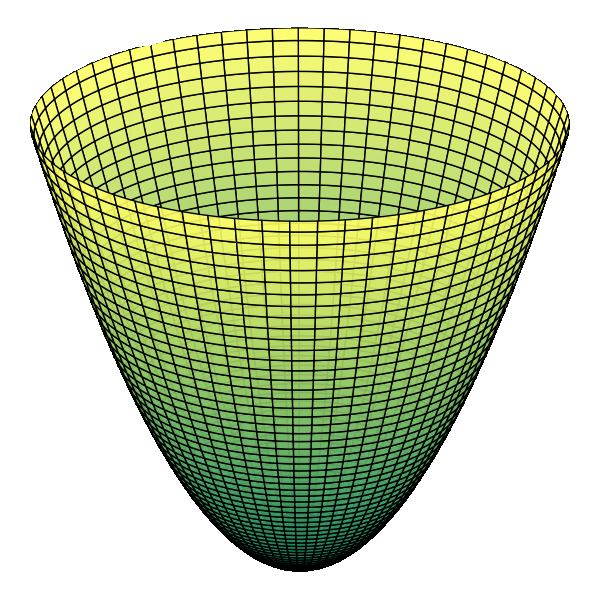
\includegraphics[width=.3\textwidth]{parabaloid.png}}}
    \subfloat{\raisebox{.2\textheight}{
\includegraphics[width=.05\textwidth]{arrow.jpg}}}
    \subfloat{{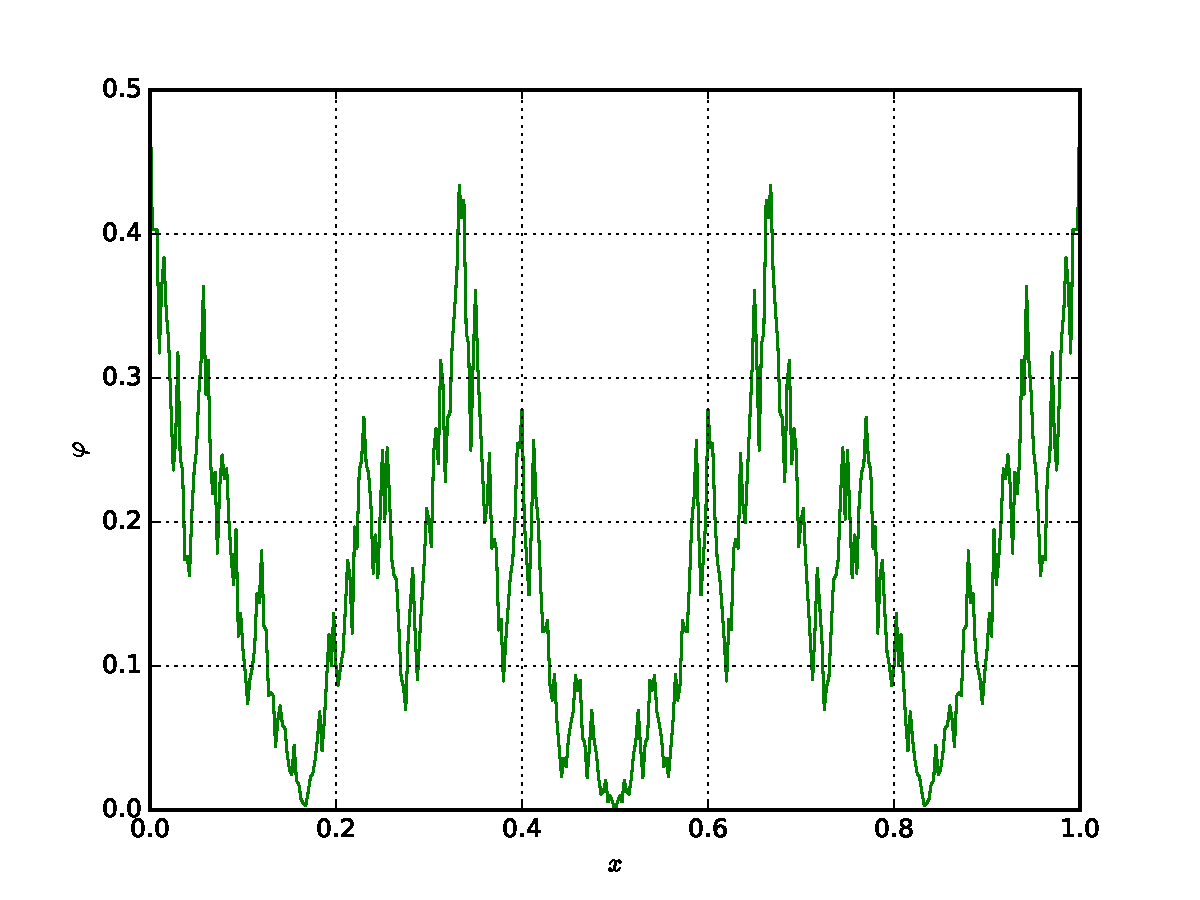
\includegraphics[width=.45\textwidth]{map_paraboloid.pdf}}}
  \end{center}
  \end{figure}
\end{frame}

\begin{frame}
  \frametitle{Smooth evolvent and non-univalent evolvent}
      %\centerline{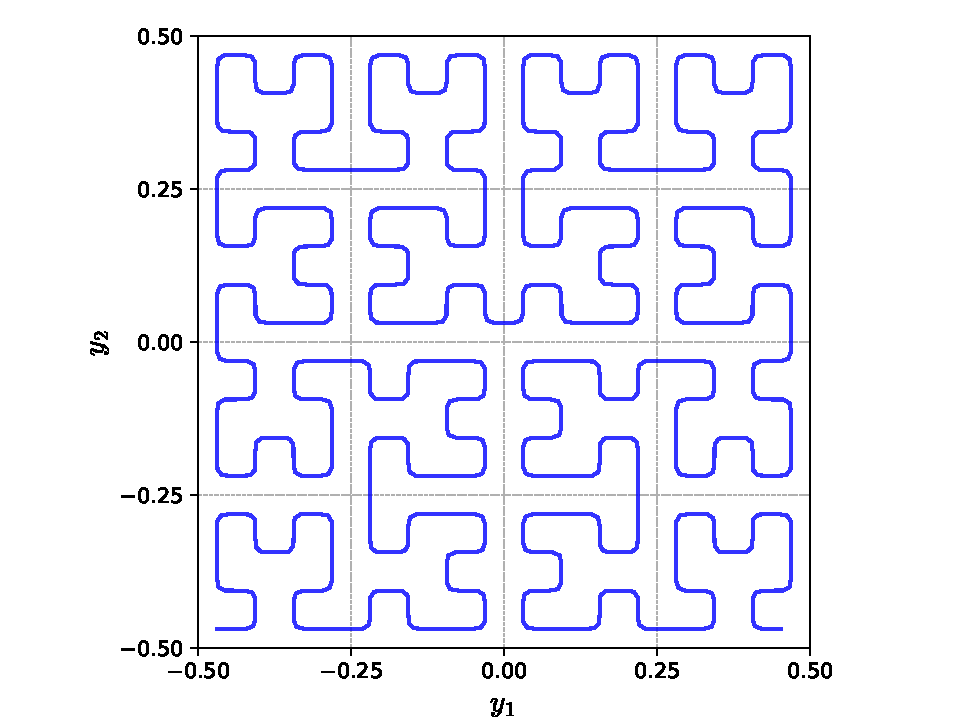
\includegraphics[width=0.9\textwidth]{smooth.pdf}}
      \begin{figure}[ht]
        %\vspace*{-0.5cm}
        \subfloat{\raisebox{.02\textheight}{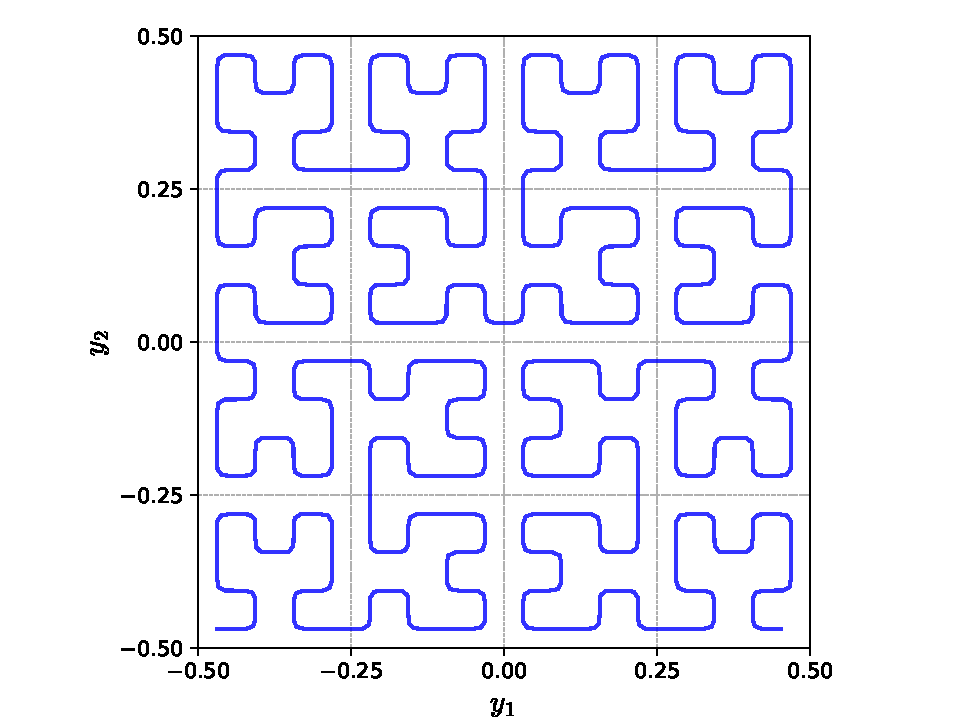
\includegraphics[width=.35\textwidth]{smooth.pdf} }}
        \subfloat{{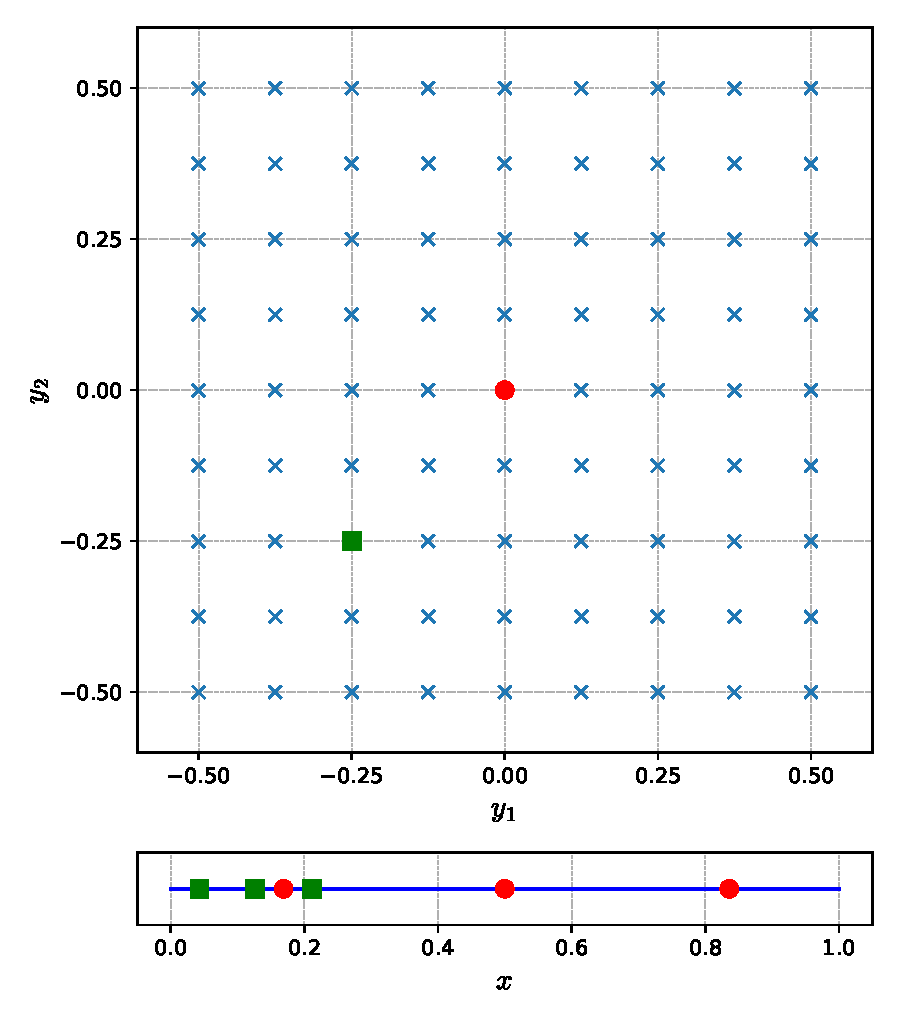
\includegraphics[width=.25\textwidth]{noninjective.pdf} }}
      \end{figure}
\end{frame}

\begin{frame}
  \frametitle{Shifted and rotated evolvents}
  \begin{figure}[ht]
    %\vspace*{-0.5cm}
    \subfloat{\raisebox{.0\textheight}{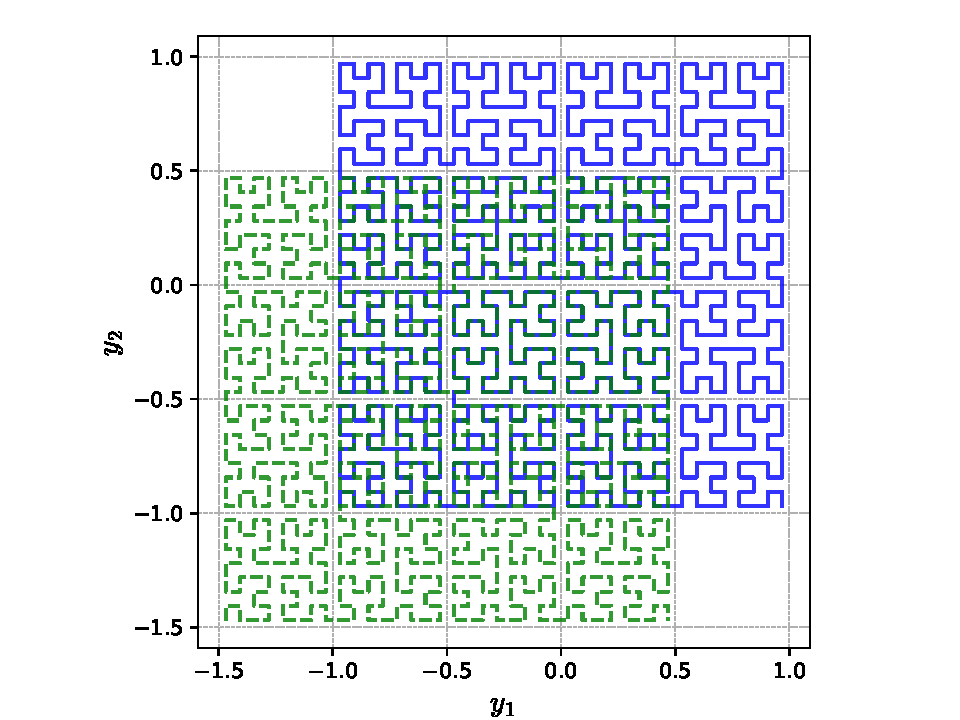
\includegraphics[width=.35\textwidth]{shifted.pdf} }}
    \subfloat{{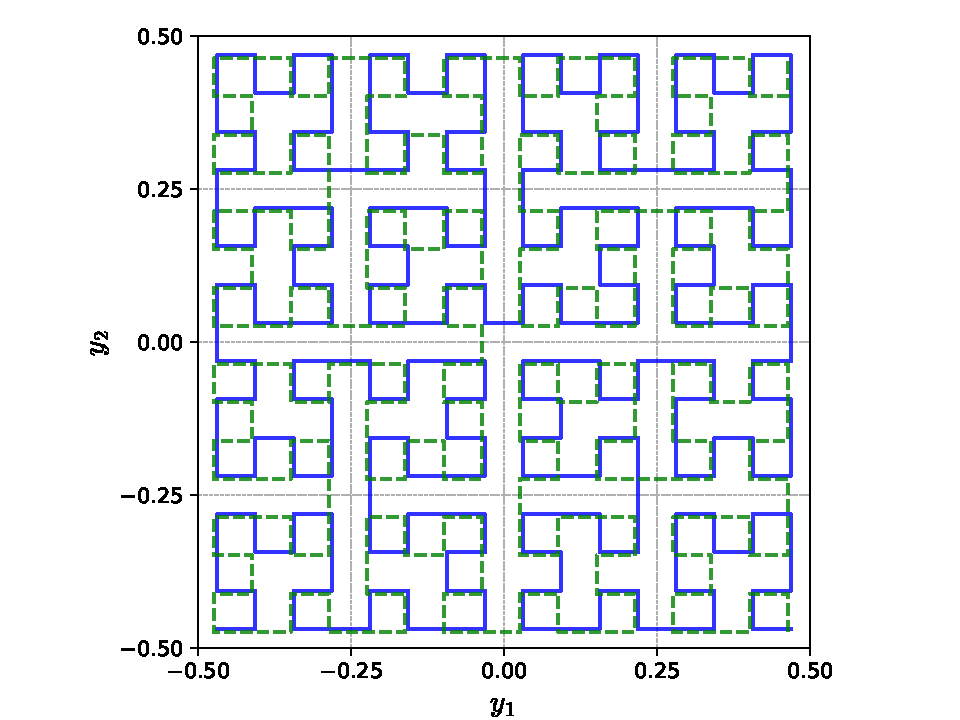
\includegraphics[width=.35\textwidth]{rotated.pdf} }}
  \end{figure}
%  \begin{columns}
%    \begin{column}{0.5\textwidth}
%
%    \end{column}
%    \begin{column}{0.5\textwidth}
%      \centerline{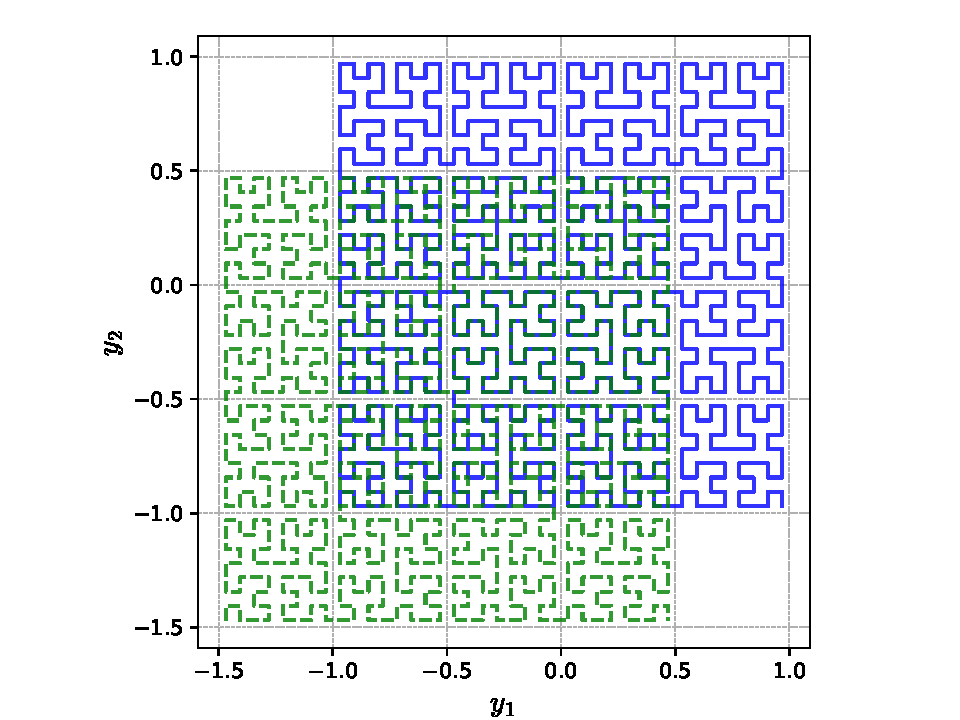
\includegraphics[width=0.9\textwidth]{shifted.pdf}}
%    \end{column}
%  \end{columns}
\end{frame}

\begin{frame}
  \frametitle{Rotated evolvent}
  \begin{columns}
    \begin{column}{0.5\textwidth}

    \end{column}
    \begin{column}{0.5\textwidth}
      \centerline{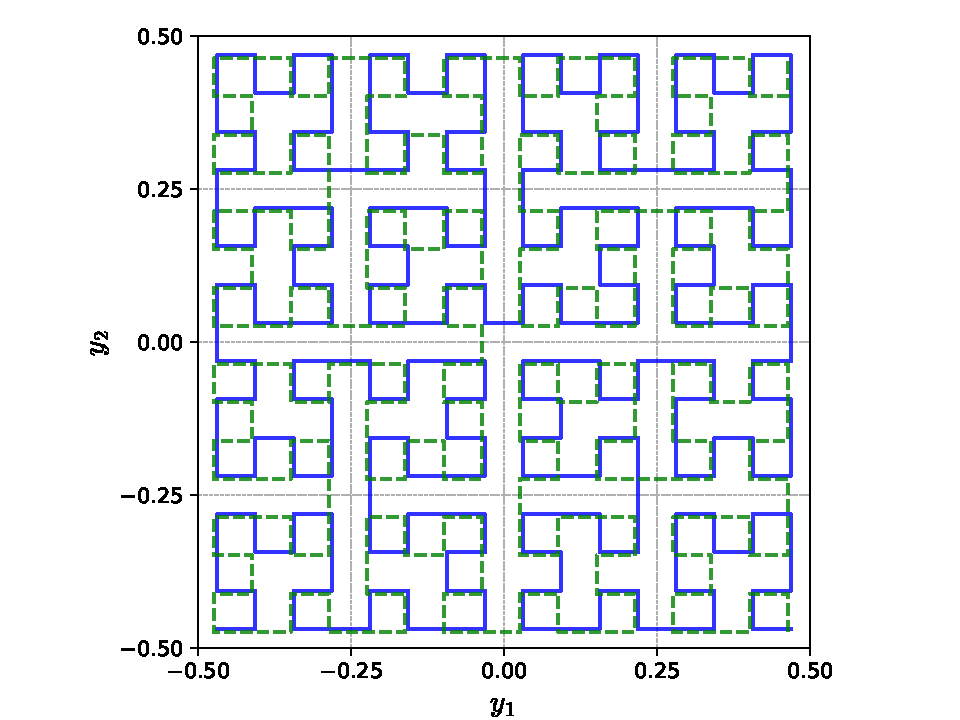
\includegraphics[width=0.9\textwidth]{rotated.pdf}}
    \end{column}
  \end{columns}
\end{frame}

\begin{frame}
  \frametitle{Optimization method}
  Optimization method generates search sequence \(\{x_k\}\) and consists of the following steps:
  \begin{enumerate}
    \setlength{\itemindent}{.1in}
    \item[Step 1.] Sort the search information (one-dimensional points) in increasing order.
    \item[Step 2.] Compute the evolvent \(y(x)\) and the function \(\varphi(y(x))\).
    \item[Step 3.] For each interval \((x_{i-1}, x_i)\) compute quantity \(R(i)\), called characteristic.
    \item[Step 4.] Choose an interval \((x_{t-1}, x_t)\) with the greatest characteristic and
    compute objective \(f(y(x))\) in the point chosen using the decision rule \(d\):
    \begin{displaymath}
      x^{k+1}=d(t)\in (x_{t-1}, x_t)
    \end{displaymath}
    \item[Step 5.] If \(x_{t}-x_{t-1}<\varepsilon\) stop the method.
  \end{enumerate}
  \textit{\footnotesize	{Detailed description: Strongin R.G., Sergeyev Ya.D.: Global optimization with non-convex constraints. Sequential and parallel algorithms (2000), Chapter 7}}
\end{frame}

\begin{frame}
  \frametitle{Test problems}
  \begin{columns}
    \begin{column}{0.5\textwidth}
      Generator GKLS was employed to construct the sets of test problems:
      \begin{displaymath}
        \begin{matrix}
          f(x)=
          \left\{
          \begin{matrix}
          C_i(x), x \in S_i, i\in 2,\dots ,m \\
          \Vert x-T \Vert^2 + t, x\not\in S_2,\dots,S_m
          \end{matrix} \right.
        \end{matrix}
      \end{displaymath}

      The generator allows to adjust:
      \begin{itemize}
        \item the number of local minimas;
        \item the size of the global minima attraction region;
        \item the space dimension.
      \end{itemize}
    \end{column}
    \begin{column}{0.5\textwidth}
      \centerline{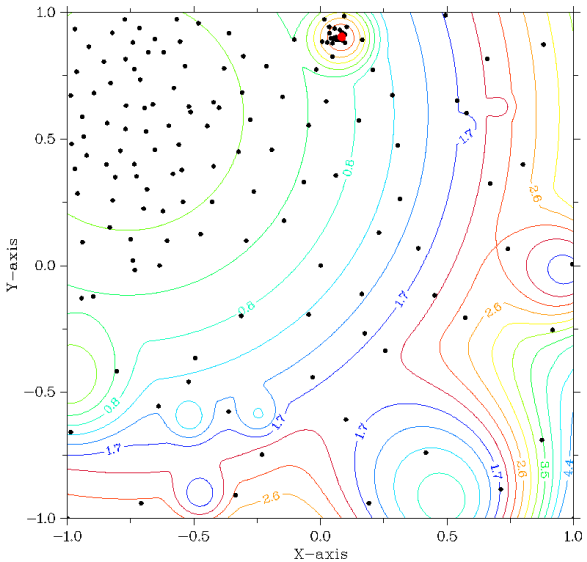
\includegraphics[width=0.9\textwidth]{gkls_color.png}}
    \end{column}
  \end{columns}
\end{frame}

\begin{frame}
  \frametitle{Results of comparison}
  \begin{figure}[ht]
    \hspace*{-0.9cm}
    \subfloat[Minimal \(r\)]{{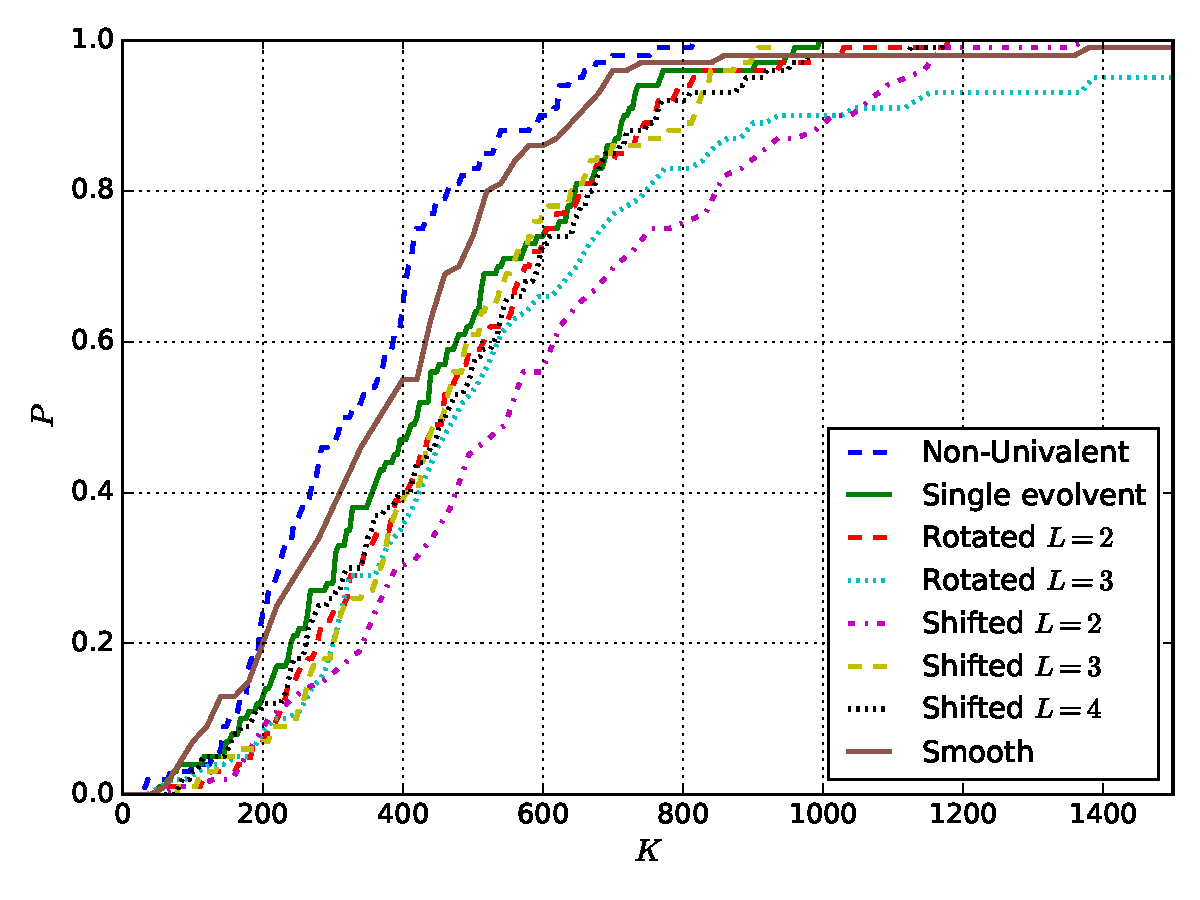
\includegraphics[width=.55\textwidth]{gklsS2d_opt_pt_op.pdf} }}
    \subfloat[\(r=5.0\)]{{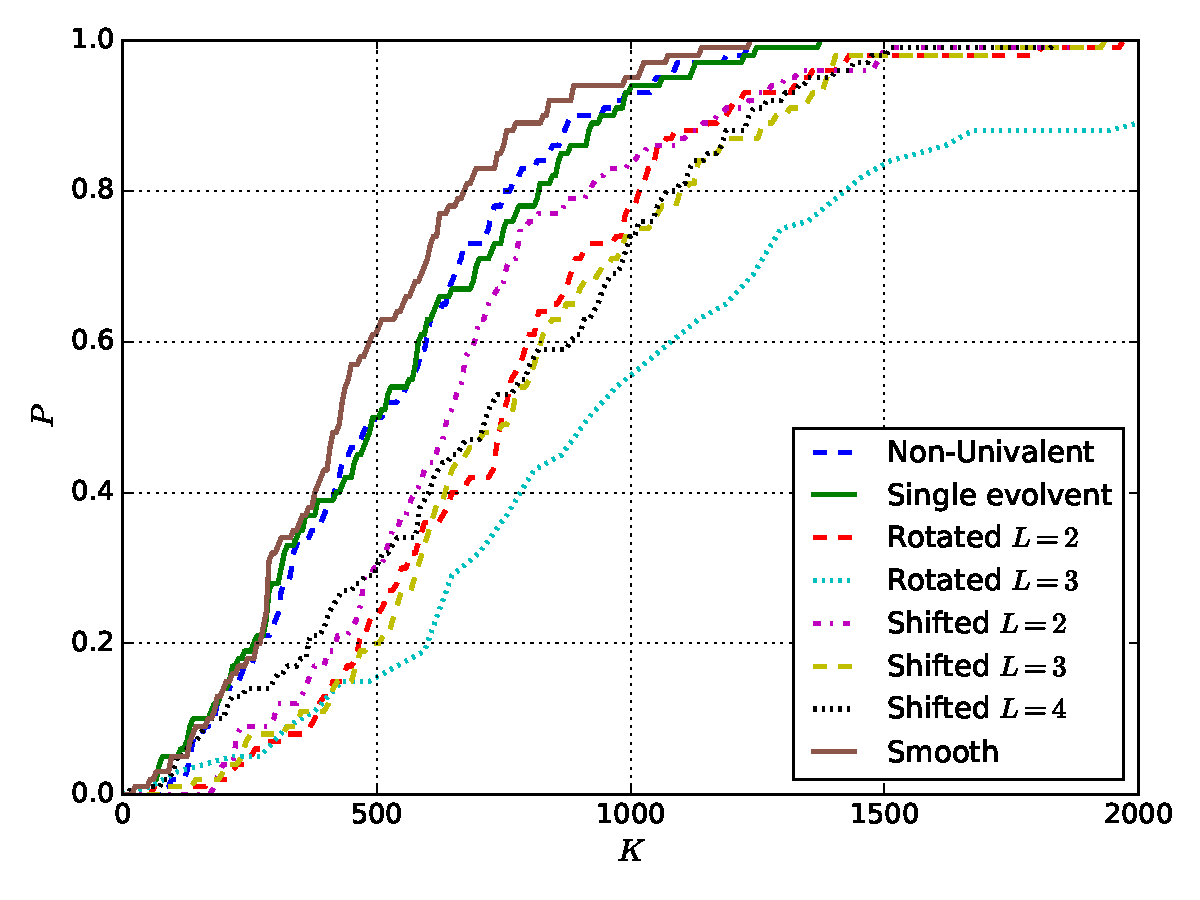
\includegraphics[width=.55\textwidth]{gklsS2d_same_r_opt_pt_op.pdf} }} \hspace*{4cm}
    \caption{Operating characteristics on GKLS 2d Simple class}
  \end{figure}
\end{frame}

\begin{frame}
  \frametitle{Results of comparison}
  \begin{figure}[ht]
    \hspace*{-0.9cm}
    \subfloat[Minimal \(r\)]{{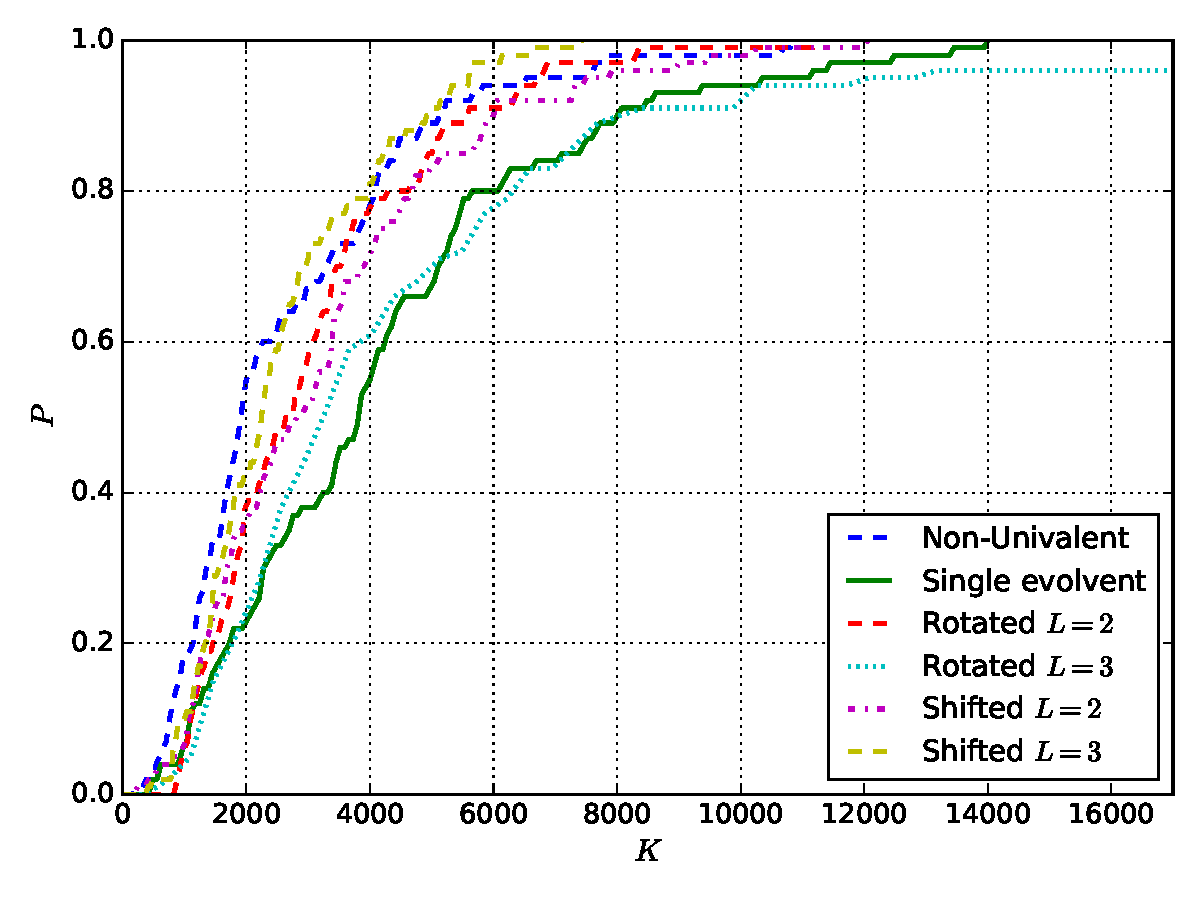
\includegraphics[width=.55\textwidth]{gklsS3d_opt_pt_op.pdf} }}
    \subfloat[\(r=4.5\)]{{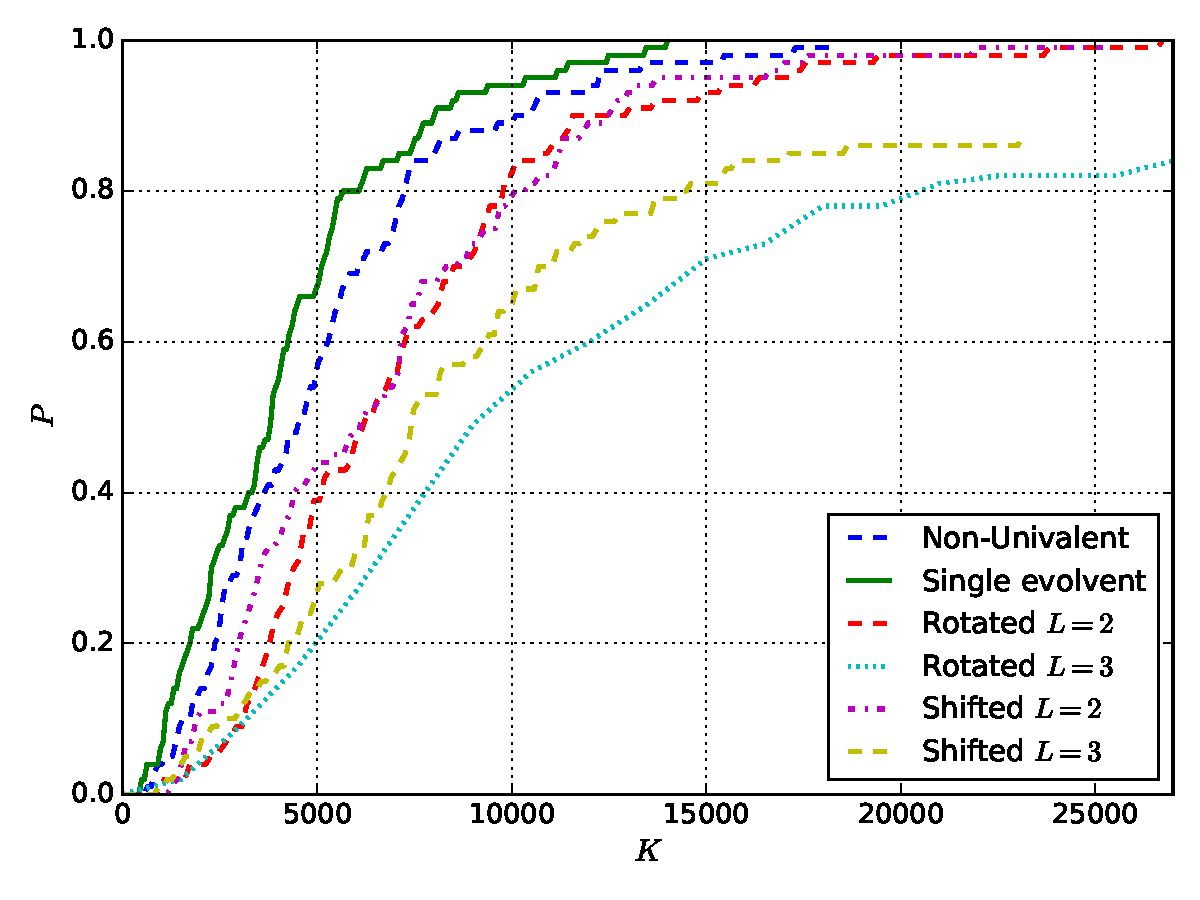
\includegraphics[width=.55\textwidth]{gklsS3d_same_r_opt_pt_op.pdf} }}
    \caption{Operating characteristics on GKLS 3d Simple class}
  \end{figure}
\end{frame}


\begin{frame}
  \frametitle{Conclusion and future work}
    Already done:
    \begin{itemize}
      \item
    \end{itemize}
    Future work:
    \begin{itemize}
      \item
    \end{itemize}
\end{frame}

\begin{frame}{{}}
  \frametitle{ }
  \begin{center}
    \Large{Q\&A}

\vspace{1cm}

    sovrasov.vlad@gmail.com

    https://github.com/sovrasov
  \end{center}
\end{frame}

\end{document}
